\section{Dreiphasen-Brückenschaltung - Ungesteuerter Betrieb}

\subsection{Messschaltung}

\begin{figure}[h!]
    \centering
    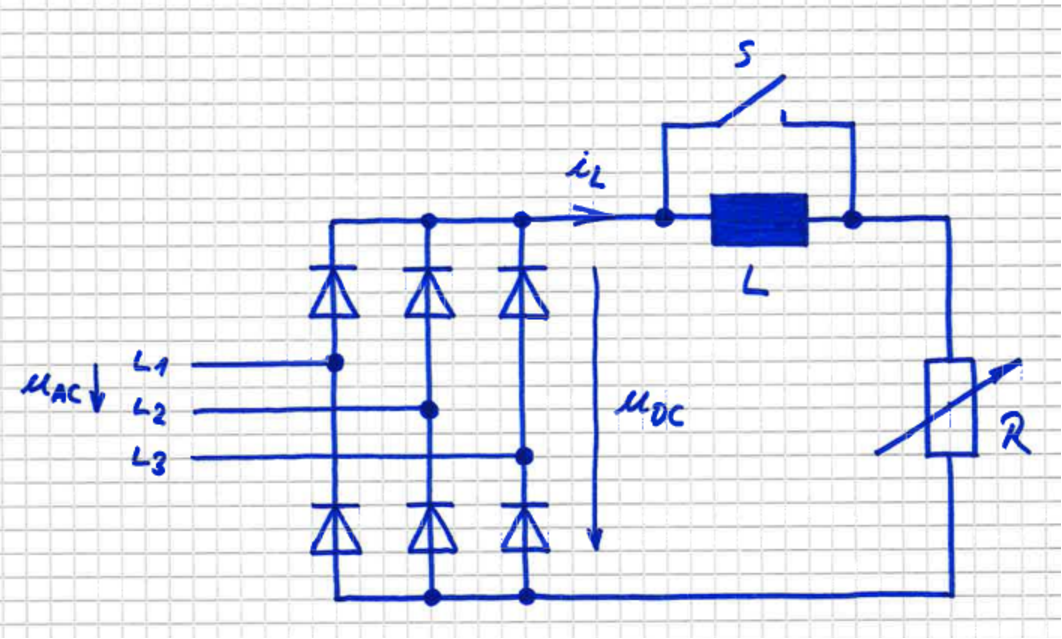
\includegraphics[scale=\sscale]{./../fig/b6_diode.pdf}
    \caption{B6 Diodengleichichter}
    \label{fig:b6_diode}
\end{figure}

\subsection{Messungen}

\begin{figure}[h!]
    \centering
    \includegraphics[scale=\pscale]{./../plots/641_01.pdf}
    \caption{B6 Diodengleichrichter mit L-Glättung, Lastposition 16}
\end{figure}

\begin{figure}[h!]
    \centering
    \includegraphics[scale=\pscale]{./../plots/641_02.pdf}
    \caption{B6 Diodengleichrichter mit L-Glättung, Lastposition 11}
\end{figure}

\begin{figure}[h!]
    \centering
    \includegraphics[scale=\pscale]{./../plots/641_03.pdf}
    \caption{B6 Diodengleichrichter mit L-Glättung, Lastposition 6}
\end{figure}

\begin{figure}[h!]
    \centering
    \includegraphics[scale=\pscale]{./../plots/641_04.pdf}
    \caption{B6 Diodengleichrichter mit L-Glättung, Lastposition 4}
\end{figure}

\clearpage
